\documentclass[reqno, a4paper]{amsart}
\newcommand\hmmax{0}
\newcommand\bmmax{0}
\usepackage{amsmath}
\usepackage{amssymb}
\usepackage{amsthm}

% PAGE DIMENSION
\usepackage[scale=0.9]{geometry}

% BIBLIOGRAPHY
\usepackage[authoryear]{natbib}
\usepackage{bibentry} % inline refereces

% ENCODING, LANGUAGE
\usepackage[czech]{babel}
\usepackage[utf8]{inputenc}

% GRAPHICS
\usepackage{graphicx}
\usepackage{wrapfig}
\usepackage{subfig}

% HYPERTEXT, SOURCE CODE SPECIALS
\usepackage[unicode]{hyperref}
\usepackage[active]{srcltx} % use TeX-souce-specials-mode

% SYMBOLS, FONTS
\usepackage{mathbbol}
\usepackage{bm} % sophisticated \boldsymbol
%\usepackage{stmaryrd}
\usepackage{MnSymbol} % \lsem, \rsem, tensor product :
\usepackage{gensymb}
\usepackage{eurosym}

% UNITS, TYPESETTING TENSORS
%\usepackage{units}
\usepackage{siunitx}
\usepackage{tensor}
\usepackage{accents}

% COMPACT LIST ENVIRONMENT
\usepackage{enumitem}

% LINE NUMBERS
\usepackage{lineno}

% TABLE OF CONTENTS IN TWO COLUMNS
% \usepackage[toc]{multitoc} % It seems that it does not work with amsart
% the workaround is the command
% \addtocontents{toc}{\protect\begin{multicols}{2}} % workaround for table of contents in two columns in amsart documentclass
% see below
\usepackage{multicol}

% TODO NOTES
\usepackage{todonotes}

% TABLES
\usepackage{booktabs}
\usepackage{dcolumn}
\usepackage{tabularx}


% SOURCE CODE LISTINGS
\usepackage{listings}
%\usepackage{minted}
\usepackage{xcolor}

% IMPORT CSV files
\usepackage{csvsimple}

% NUMBERS
%\usepackage{numprint}

\numberwithin{equation}{section}
\let\cite\citet
\newcommand*{\doi}[1]{\href{http://dx.doi.org/#1}{doi: #1}}

%\makeatletter
% \@ifpackageloaded{tensor}% tensor is a package for a better typesetting of tensors
% {
% \renewcommand{\tnsr@Aux}[3][]{%
% \mathpalette{\tnsr@Plt{#1}{#3}}{\mathrm #2}%
% \tnsr@Wrn
% }%\tnsr@Aux
% }{%
% \relax%
% }
% \makeatother


% operators
\DeclareMathOperator{\divergence}{div}
\DeclareMathOperator{\Divergence}{Div}
\DeclareMathOperator{\gradient}{grad}
\DeclareMathOperator{\Gradient}{Grad}
\DeclareMathOperator{\rot}{rot}
\DeclareMathOperator{\Asym}{Asym}
\DeclareMathOperator{\Sym}{Sym}
\DeclareMathOperator{\Tr}{Tr}
\DeclareMathOperator{\signum}{sign}
\DeclareMathOperator{\supp}{supp}
\DeclareMathOperator{\cof}{cof} % cofactor
\DeclareMathOperator{\residue}{res}
\DeclareMathOperator{\ad}{ad} % adjoint ad_X (Y) = [X,Y]  
\DeclareMathOperator{\distanceop}{dist} % distance in a metric space

% Kernel, range, rank
\DeclareMathOperator{\kernelop}{{\mathcal N}}
\DeclareMathOperator{\rangeop}{{\mathcal R}}
\DeclareMathOperator{\rankop}{rank}

% jump
\newcommand{\jumpdis}[1]{\ensuremath{\left\lsem #1 \right\rsem}} % difference between function values at the point of jump discontinuity

% hyperbolic functions
\DeclareMathOperator{\arcsinh}{arcsinh}
\DeclareMathOperator{\arccosh}{arccosh}
\DeclareMathOperator{\arctanh}{arctanh}
\DeclareMathOperator{\arccoth}{arccoth}

% invariants of second order tensor
\DeclareMathOperator{\invariantI}{I_1}
\DeclareMathOperator{\invariantII}{I_2}
\DeclareMathOperator{\invariantIII}{I_3}

% big o
\newcommand{\bigo}[1]{\ensuremath{O\left(#1 \right)}}
\newcommand{\smallo}[1]{\ensuremath{o\left(#1 \right)}}

% exponential
\newcommand{\exponential}[1]{\ensuremath{{\mathrm e}^{#1}}}

% imaginary unit
\newcommand{\iunit}{\ensuremath{\mathrm{i}}}


% real and imaginary part
\newcommand{\realp}{\mathrm{real}}
\newcommand{\imagp}{\mathrm{imag}}

%\newcommand{\Real}{\Re}
%\newcommand{\Imag}{\Im}
\providecommand{\Real}{\Re}
\providecommand{\Imag}{\Im}

% predicates
\newcommand{\charac}{\ensuremath{\mathrm{char}}} % characteristic quantity such as length scale, etc.
\newcommand{\reference}{\mathrm{ref}}
\newcommand{\crit}{\mathrm{crit}}
\newcommand{\bydefinition}{\mathrm{def}}
\newcommand{\traceless}[1]{{#1}_{\delta}}

% dimensionless variables and functions
\newcommand{\dimless}[1]{#1^\star}

% derivatives
\newcommand{\diff}{\mathrm{d}}
\newcommand{\Diff}[1][]{\mathrm{D}_{#1}} % For Frechet and Gateaux derivative
\newcommand{\hDiff}[2][]{\mathrm{D}^{#1}_{#2}} % Higher order Frechet and Gateaux derivative

% inexact differential
\newcommand{\dbar}{{\mathchar'26\mkern-12mu \diff}}
\newcommand{\idiff}{\dbar}

% body
\newcommand{\body}{{\mathcal B}}

% vectors and tensors
\renewcommand{\vec}[1]{\ensuremath{\mathbf{#1}}}
\newcommand{\greekvec}[1]{\ensuremath{\boldsymbol{#1}}}
\makeatletter
\@ifpackageloaded{bm}% 
{\renewcommand{\vec}[1]{\ensuremath{\bm{#1}}}%
\renewcommand{\greekvec}[1]{\ensuremath{\bm{#1}}}%
}{%
\relax% do nothing
}
\makeatother
\newcommand{\tensorq}[1]{\ensuremath{\mathbb{#1}}}      % tensorial quantity
\newcommand{\tensorc}[1]{\ensuremath{\mathrm{#1}}}      % tensorial quantity components  

\newcommand{\conjugate}[1]{#1^\star}
\newcommand{\transpose}[1]{#1^\top}
\newcommand{\transposei}[1]{#1^{-\top}}
\newcommand{\inverse}[1]{#1^{-1}}

% Identity matrix and zero matrix
\newcommand{\identity}{\ensuremath{\tensorq{I}}} % identity
\newcommand{\tensorzero}{{\mathbb{O}}} % zero tensor

% Cauchy stress
\newcommand{\cstress}{\tensorq{T}}
\newcommand{\cstressc}{\tensorc{T}}

% Cauchy stress, thermodynamically determined part
%\DeclareMathSymbol{\robustrho}{\mathord}{letters}{"1A} % If I want to write \fid{\thcstressrho} it sometimes happes that the greek letters in subscript get crippled, this happens expecially in MDPI class. This tirck protects \rho. It would work also for other greek letters, the codes are given in  fontdef.dtx
\newcommand{\thcstress}{\ensuremath{\cstress_{\mathrm{th}}}} 
%\newcommand{\thcstressrho}{\ensuremath{\cstress_{\mathrm{th},\, \robustrho}}} % thermodynamically determined part divided by rho
\newcommand{\thcstressrho}{\ensuremath{\cstress_{\mathrm{th},\, \mathnormal{\rho}}}} % thermodynamically determined part divided by rho
\newcommand{\tracelessthcstress}{\traceless{\left(\thcstress\right)}} % traceless part
\newcommand{\tracelessthcstressrho}{\traceless{\left(\cstress_{\mathrm{th},\, \rho}\right)}} % traceless part divided by rho

% Extra stress tensor
\newcommand{\ecstress}{\tensorq{S}}
\newcommand{\ecstressc}{\tensorc{S}}

% First Piola stress tensor
\newcommand{\fpstress}{\tensorq{T}_{\mathrm{R}}}
\newcommand{\fpstressc}{\tensorc{T}_{\mathrm R}}

% Second Piola--Kirchhoff stress tensor
\newcommand{\spstress}{\tensorq{S}_{\mathrm{R}}}
\newcommand{\spstressc}{\ensuremath{{{\mathrm S}_{\mathrm R}}}}

% Couple stress tensor
\newcommand{\couplestress}{\tensorq{M}}
\newcommand{\couplestressc}{\tensorc{M}}

% deformation, deformation gradient
\newcommand{\deformation}{\greekvec{\chi}}
\newcommand{\deformationc}{\tensorc{\chi}}

\newcommand{\fgrad}{\tensorq{F}}
\newcommand{\fgradc}{\tensorc{F}}
\newcommand{\fgradrel}[3][]{\fgrad^{#1}_{#2}\left(#3\right)}

% determinant of deformation gradient, Jacobian
\newcommand{\detfgrad}{J}

% displacement
\newcommand{\displacement}{\vec{U}}
\newcommand{\displacementc}{\tensorc{U}}

% right Cauchy-Green tensor
\newcommand{\rcg}{\tensorq{C}}
\newcommand{\rcgc}{\tensorc{C}}        
\newcommand{\rcgrel}[3][]{\rcg^{#1}_{#2}\left(#3\right)}

% left Cauchy-Green tensor
\newcommand{\lcg}{\tensorq{B}}
\newcommand{\lcgc}{\tensorc{B}}        
\newcommand{\lcgrel}[3][]{\lcg^{#1}_{#2}\left(#3\right)}
\newcommand{\lcgb}{\overline{\lcg}} % rescaled left Cauchy--Green tensor, theory of slightly compressible materials
\newcommand{\lcgbc}{\overline{\lcgc}} % rescaled left Cauchy--Green tensor, theory of slightly compressible materials, components


%\newcommand{\piolastrain}{\tensorq{b}} % Piola deformation tensor (inverse of right Cauchy--Green)
%\newcommand{\fingerstrain}{\tensorq{c}} % Finger deformation tensor (inverse of left Cauchy--Green)

% rotation
\newcommand{\rotation}{\tensorq{R}}
\newcommand{\rotationrel}[3][]{\rotation^{#1}_{#2}\left(#3\right)}

% stretch
\newcommand{\stretchu}{\tensorq{U}}
\newcommand{\stretchurel}[3][]{\stretchu^{#1}_{#2}\left(#3\right)}
\newcommand{\stretchv}{\tensorq{V}}
\newcommand{\stretchvrel}[3][]{\stretchv^{#1}_{#2}\left(#3\right)}

% linearized strain (symmetric part of displacement gradient), skew-symmetric part of displacement gradient
\makeatletter
\@ifpackageloaded{bm}% 
{%
\newcommand{\linstrain}{\bbespilon} %requires \usepackage[bbgreekl]{mathbbol}
% YES, the spelling is wrong, but this is how it is coded in the package
}{%
\newcommand{\linstrain}{\tensorq{\varepsilon}}
}

\@ifpackageloaded{bm}%
{%
\newcommand{\skewdgradient}{\bbomega} 
}{%
\newcommand{\skewdgradient}{\tensorq{\omega}}
}

\@ifpackageloaded{bm}%
{%
\newcommand{\linstress}{\bbtau} % stress in linearised elasticity
}{%
\newcommand{\linstress}{\tensorq{\tau}}
}
\makeatother

\newcommand{\linstrainc}{\mathrm{\varepsilon}}
\newcommand{\linstressc}{\mathrm{\tau}}
\newcommand{\skewdgradientc}{\mathrm{\omega}}

% Lagrangean and Eulerian strain
\newcommand{\lstrain}{\tensorq{E}} % Green--Saint-Venant strain
\newcommand{\lstrainc}{\tensorc{E}} % Green--Saint-Venant strain, components
\newcommand{\estrain}{\tensorq{e}} % Euler--Almansi strain, components
\newcommand{\estrainc}{\tensorc{e}} % Euler--Almansi strain, components

% Hencky strain
\newcommand{\henckystrain}{\tensorq{H}} % Hencky strain
\newcommand{\henckystrainc}{\tensorc{H}} % Hencky strain, components

\newcommand{\devhencky}{\overline{\tensorq{H}}} % Hencky strain, deviatoric part via deviatoric deformation
\newcommand{\devhenckyc}{\overline{\tensorc{H}}} % Hencky strain, deviatoric part via deviatoric deformation, components


% Rivlin-Ericksen tensor
\newcommand{\rivlin}{{\tensorq{A}}}

% generic tensor quantity
\newcommand{\generictensor}{{\tensorq{A}}}
\newcommand{\generictensorc}{\tensorc{A}} % component of the tensor

% deviatoric part of Cauchy stress
\newcommand{\dcstress}{\cstress - \left( \frac{1}{3}\Tr \cstress \right) \identity}
\newcommand{\dcstresssymb}{\traceless{\cstress}}

% mean normal stress
\newcommand{\cstressnorm}{\frac{1}{3}\Tr \cstress}

% velocity and velocity gradient, (skew)symmetric part of velocity gradient
\newcommand{\vecv}{\ensuremath{\vec{v}}}
\newcommand{\gradv}{\ensuremath{\nabla \vecv}}
\newcommand{\gradasym}{\ensuremath{\tensorq{W}}}
\newcommand{\gradsym}{\ensuremath{\tensorq{D}}}
\newcommand{\dgradsymsymb}{\ensuremath{\gradsym_{\delta}}}
\newcommand{\gradvl}{\ensuremath{\tensorq{L}}}

% surface velocity
\newcommand{\unders}[1]{\ensuremath{\underaccent{\mathrm{s}}{#1}}}

\newcommand{\gradsymop}{\nabla_{\mathrm{sym}}}
\newcommand{\gradasymop}{\nabla_{\mathrm{asym}}}

\newcommand{\vecvc}{\tensorc{v}}

% velocity and velocity gradient, (skew)symmetric part of velocity gradient, COMPONENTS
\newcommand{\gradsymc}{\tensorc{D}}
\newcommand{\gradasymc}{\tensorc{W}}

% functionals
\newcommand{\functional}[1]{{\mathfrak #1}}
\newcommand{\fhistory}[3]{{\functional{#1}_{#2}^{#3}}}

% base vectors
\newcommand{\bvec}[1]{\vec{e}_{#1}} % current configuration
\newcommand{\Bvec}[1]{\vec{E}_{#1}} % reference configuration

% dual base vectors
\newcommand{\bvecd}[1]{\vec{e}^{#1}} % current configuration
\newcommand{\Bvecd}[1]{\vec{E}^{#1}} % reference configuration

% Cartesian basis, current configuration
\newcommand{\bvecx}{\bvec{\hat{x}}}
\newcommand{\bvecy}{\bvec{\hat{y}}}
\newcommand{\bvecz}{\bvec{\hat{z}}}

% Cartesian basis, reference configuration
\newcommand{\BvecX}{\Bvec{\hat{X}}}
\newcommand{\BvecY}{\Bvec{\hat{Y}}}
\newcommand{\BvecZ}{\Bvec{\hat{Z}}}

% Cartesian dual basis, reference configuration
\newcommand{\BvecdX}{\Bvecd{\hat{X}}}
\newcommand{\BvecdY}{\Bvecd{\hat{Y}}}
\newcommand{\BvecdZ}{\Bvecd{\hat{Z}}}

% Cartesian dual basis, current configuration
\newcommand{\bvecdx}{\bvecd{\hat{x}}}
\newcommand{\bvecdy}{\bvecd{\hat{y}}}
\newcommand{\bvecdz}{\bvecd{\hat{z}}}

% same as above but now in cylindrical coordinates
\newcommand{\bvecr}{\bvec{\hat{r}}}
\newcommand{\bvect}{\bvec{\hat{\theta}}}
\newcommand{\bvecp}{\bvec{\hat{\varphi}}}
%\newcommand{\bvecz}{\bvec{\hat{z}}}

\newcommand{\bvecdr}{\bvecd{\hat{r}}}
\newcommand{\bvecdt}{\bvecd{\hat{\theta}}}
\newcommand{\bvecdp}{\bvecd{\hat{\varphi}}}

\newcommand{\BvecR}{\Bvec{\hat{R}}}
\newcommand{\BvecP}{\Bvec{\hat{\Phi}}}
%\newcommand{\BvecZ}{\Bvec{\hat{Z}}}

\newcommand{\BvecdR}{\Bvecd{\hat{R}}}
\newcommand{\BvecdP}{\Bvecd{\hat{\Phi}}}
%\newcommand{\BvecdZ}{\Bvecd{\hat{Z}}}

% components
\newcommand{\vhatx}[1][\vecvc]{{#1}^{\hat{x}}}
\newcommand{\vhaty}[1][\vecvc]{{#1}^{\hat{y}}}
%\newcommand{\bvhatz}{\vhat{e}_{\hat{z}}}

\newcommand{\vhatr}[1][\vecvc]{{#1}^{\hat{r}}}
\newcommand{\vhatt}[1][\vecvc]{{#1}^{\hat{\theta}}}
\newcommand{\vhatp}[1][\vecvc]{{#1}^{\hat{\varphi}}}
\newcommand{\vhatz}[1][\vecvc]{{#1}^{\hat{z}}}

% indices
\newcommand{\hatx}{\hat{x}}
\newcommand{\haty}{\hat{y}}
\newcommand{\hatz}{\hat{z}}
\newcommand{\hatr}{\hat{r}}
\newcommand{\hatp}{\hat{\varphi}}
\newcommand{\hatt}{\hat{\theta}}
\newcommand{\hatX}{\hat{X}}
\newcommand{\hatY}{\hat{Y}}
\newcommand{\hatZ}{\hat{Z}}

% inner and outer radius (for some calcualtions)
\newcommand{\Rin}{R_{\mathrm{in}}}
\newcommand{\Rout}{R_{\mathrm{out}}}
\newcommand{\rin}{r_{\mathrm{in}}}
\newcommand{\rout}{r_{\mathrm{out}}}
 
% base vectors, abstract covariant and contravariant basis, current configuration
\newcommand{\cobvec}[1]{\vec{g}_{#1}} % covariant base vector
\newcommand{\conbvec}[1]{\vec{g}^{#1}} % contravariant base vector
\newcommand{\cobvecn}[1]{\vec{g}_{\hat{#1}}} % covariant base vector
\newcommand{\conbvecn}[1]{\vec{g}^{\hat{#1}}} % contravariant base vector

% base vectors, abstract covariant and contravariant basis, reference configuration
\newcommand{\coBvec}[1]{\vec{G}_{#1}} % covariant base vector
\newcommand{\conBvec}[1]{\vec{G}^{#1}} % contravariant base vector
\newcommand{\coBvecn}[1]{\vec{G}_{\hat{#1}}} % covariant base vector
\newcommand{\conBvecn}[1]{\vec{G}^{\hat{#1}}} % contravariant base vector

% current configuration
\newcommand{\mtensor}{\tensorq{g}}  % metric tensor
\newcommand{\mtensorc}{{\mathrm g}} % metric tensor, components

% reference configuration
\newcommand{\mTensor}{\tensorq{G}}  % metric tensor
\newcommand{\mTensorc}{{\mathrm G}} % metric tensor, components

% Christoffel symbols
\newcommand{\christoffel}[2]{\tensor{\Gamma}{^{#1}_{#2}}}

% mean curvature
\newcommand{\meancurvature}{\mathrm{K}} % mean curvature

\newcommand{\mtensorref}{\tensorq{G}}  %metric tensor in reference configuration
\newcommand{\mtensorrefc}{{\mathrm G}} %metric tensor in reference configuration, components

% Kronecker delta, Levi--Civitta symbol
\newcommand{\kdelta}[1]{\tensor{\delta}{#1}}
\newcommand{\lcepsilon}[1]{\tensor{\epsilon}{#1}}

% distributions
\newcommand{\diracdelta}{\delta}
\newcommand{\Heaviside}{H}

% hypergeometric function
\newcommand{\hypergeom}[4]{\ensuremath{ \mathrm{F}\left( \left[#1, #2 \right]; \left[ #3 \right]; #4\right)}}

% sets
\newcommand{\R}{\ensuremath{{\mathbb R}}}
\makeatletter
%\@ifpackageloaded{hyperref}% \C is defined in hyperref package
%{\renewcommand{\C}{\ensuremath{{\mathbb C}}}%
%}{%
%\newcommand{\C}{\ensuremath{{\mathbb C}}}%
%}
\makeatother
%\renewcommand{\C}{\ensuremath{{\mathbb C}}}% The lines above are no longer needed?
\newcommand{\Q}{\ensuremath{{\mathbb Q}}}
\newcommand{\N}{\ensuremath{{\mathbb N}}}
\newcommand{\Z}{\ensuremath{{\mathbb Z}}}


% Reynolds, Womersley number, etc.
\newcommand{\Reynolds}{\mathrm{Re}}
\newcommand{\Womersley}{\mathrm{Wo}}
\newcommand{\Rayleigh}{\mathrm{Ra}}
\newcommand{\RayleighSqrt}{\mathrm{R}}
\newcommand{\Prandtl}{\mathrm{Pr}}
\newcommand{\Grashof}{\mathrm{Gr}}
\newcommand{\Mach}{\mathrm{Ma}}
\newcommand{\Froude}{\mathrm{Fr}}
\newcommand{\Peclet}{\mathrm{Pe}}
\newcommand{\Eckert}{\mathrm{Ec}}
\newcommand{\Brinkman}{\mathrm{Br}}
\newcommand{\Nusselt}{\mathrm{Nu}}

% Young modulus, Poisson ratio
\newcommand{\Young}{\mathrm{E}}
\newcommand{\Poisson}{\mathrm{\nu}}

% bulk modulus, shear modulus
\newcommand{\bulkm}{\mathrm{K}}
\newcommand{\shearm}{\mathrm{G}}

% Symetric and antisymetric tensors
\newcommand{\asym}[1]{\ensuremath{\Asym \left( #1 \right)}}
\newcommand{\sym}[1]{\ensuremath{\Sym \left( #1 \right)}}

% Energy, free energy, entropy, temperature
\newcommand{\tenergy}{\ensuremath{e}_{\mathrm{tot}}} % specific total energy (energy per unit mass), sum of specific internal energy and the specific kinetic energy
\newcommand{\ienergy}{\ensuremath{e}} % specific internal energy (energy per unit mass)
\newcommand{\menergy}{\ensuremath{e}_{\mathrm{mech}}} % specific mechanical energy (energy per unit mass), kinetic energy plus internal energy minus thermal contribution
\newcommand{\kenergy}{\ensuremath{e_{\mathrm{kin}}}} % specific kinetic energy (kinetic energy per unit mass)
\newcommand{\fenergy}{\ensuremath{\psi}} % specific free energy
\newcommand{\entropy}{\ensuremath{\eta}} % specific entropy
\newcommand{\entalphy}{\ensuremath{h}} % specific enthalpy
\newcommand{\gibbs}{\ensuremath{g}} % specific Gibbs free energy

\newcommand{\temp}{\ensuremath{\theta}} % temperature, Eulerian description
\newcommand{\Temp}{\ensuremath{\Theta}} % temperature, Lagrangian description
\newcommand{\thpressure}{\ensuremath{p_{\mathrm{th}}}} % thermodynamic pressure

\newcommand{\mns}{\ensuremath{m}} % mean normal stress
\newcommand{\temptoref}{\ensuremath{\vartheta}} % (temperature - reference temperature)/(reference temperature)

% Net energy, free energy, entropy, ...
\newcommand{\nettenergy}{\ensuremath{E}_{\mathrm{tot}}} % net total energy
\newcommand{\netmenergy}{\ensuremath{E}_{\mathrm{mech}}} % net mechanical energy
\newcommand{\netthenergy}{\ensuremath{E}_{\mathrm{therm}}} % net thermal energy
\newcommand{\netienergy}{\ensuremath{E}} % net internal energy
\newcommand{\netkenergy}{\ensuremath{E_{\mathrm{kin}}}} % net kinetic energy
\newcommand{\netentropy}{\ensuremath{S}} % net entropy
\newcommand{\netheat}{\ensuremath{Q}} % net heat

% Specific molar gas constant
\newcommand{\Rspecific}{\ensuremath{R_{\mathrm{s}}}}
\newcommand{\Rmol}{\ensuremath{R_{\mathrm{m}}}}
 
% Specific heat at constant volume 
\newcommand{\cheatvol}{\ensuremath{c_{\mathrm{V}}}}
\newcommand{\cheatvolref}{\ensuremath{c_{\mathrm{V}, \reference}}} % reference value

% Specific heat at constant pressure 
\newcommand{\cheatpressure}{\ensuremath{c_{\mathrm{P}}}}
\newcommand{\cheatpressureref}{\ensuremath{c_{\mathrm{P}, \reference}}} % reference value

% Density in reference configuration
\newcommand{\rhor}{\rho_{\mathrm{R}}}

% Energy flux, heat flux, entropy flux
\newcommand{\efluxc}{\vec{j}_{e}} % energy flux, current configuration
\newcommand{\eflux}{\vec{J}_{e}} % energy flux, reference configuration

\newcommand{\hfluxc}{\vec{j}_{q}}     % heat flux, current configuration
\newcommand{\hfluxcc}{\tensorc{j}_{q}}     % heat flux, current configuration, components
\newcommand{\hflux}{\vec{J}_{q}}     % heat flux, reference configuration

\newcommand{\entfluxc}{\vec{j}_{\entropy}} % entropy flux, current configurtion 
\newcommand{\entflux}{\vec{J}_{\entropy}} % entropy flux, reference configuration

% Energy source, entropy source
\newcommand{\esourcec}{\ensuremath{q_{e}}} % energy source, current configuration
\newcommand{\hsourcec}{\ensuremath{q}} % heat source, current configuration
\newcommand{\entsourcec}{\ensuremath{q_{\entropy}}} % entropy source, current configuration

% Thermodynamical fluxes and affinities
\newcommand{\thfluxc}[1]{\vec{j}_{#1}} % thermodynamic flux, current configuration
\newcommand{\thaffinityc}[1]{\vec{a}_{#1}} % thermodynamic affinity, current configuration

% Entropy production
\newcommand{\entprodc}{\xi} % entropy production, current configuration
%  The entropy evolution equation is written as \rho \dd{\entropy}{t} + \divx \entfluxc = \entprodc
\newcommand{\entprodctemp}{\zeta} % entropy production times temperature, current configuration

% Derivatives, partial derivatives, covariant derivatives 
\newcommand{\pd}[2]{\ensuremath{\frac{\partial {#1}}{\partial {#2}}}}
\newcommand{\ppd}[2]{\ensuremath{\frac{\partial^2 {#1}}{\partial {#2^2}}}}
\newcommand{\dd}[2]{\ensuremath{\frac{\diff {#1}}{\diff {#2}}}}
\newcommand{\cd}[2]{\ensuremath{\frac{\diff^* {#1}}{\diff {#2}}}}
\newcommand{\ddd}[2]{\ensuremath{\frac{\diff^2 {#1}}{\diff {#2}^2}}}

% Upper convected (Oldroyd) derivative
\newcommand{\fid}[1]{\ensuremath{\accentset{\triangledown}{#1}}}
\newcommand{\fidd}[1]{\ensuremath{\accentset{\triangledown \! \triangledown}{#1}}}

% Lower convected derivative
\newcommand{\lfid}[1]{\ensuremath{\accentset{\meddiamond}{#1}}}
\newcommand{\lfidd}[1]{\ensuremath{\accentset{\meddiamond \! \meddiamond}{#1}}}

% Jaumann derivative
\newcommand{\jfid}[1]{\ensuremath{\accentset{\vartriangle}{#1}}}
\newcommand{\jfidd}[1]{\ensuremath{\accentset{\vartriangle \! \vartriangle}{#1}}}

% Green--Naghdi derivative
\newcommand{\gfid}[1]{\ensuremath{\accentset{\medsquare}{#1}}}
\newcommand{\gfidd}[1]{\ensuremath{\accentset{\medsquare \! \medsquare}{#1}}}

% Truesdell derivative
\newcommand{\tfid}[1]{\ensuremath{\accentset{\medcircle}{#1}}}
\newcommand{\tfidd}[1]{\ensuremath{\accentset{\medcircle \! \medcircle}{#1}}}

% Material derivative (\dot with \overline)
\newcommand{\mdif}[1]{\ensuremath{\dot{\overline{#1}}}}

\makeatletter
\@ifpackageloaded{tensor}% tensor is a package for a better typesetting of tensors
{
\newcommand{\codev}[2]{\ensuremath{\left. {#1} \right|\indices{_{#2}}}}
}{%
\newcommand{\codev}[2]{\ensuremath{\left. {#1} \right|_{#2}}}
}
\makeatother

\makeatletter
\@ifpackageloaded{tensor}% tensor is a package for a better typesetting of tensors
{
\newcommand{\contradev}[2]{\ensuremath{\left. {#1} \right|\indices{^{#2}}}}
}{%
\newcommand{\contradev}[2]{\ensuremath{\left. {#1} \right|^{#2}}}
}
\makeatother


% Bessel and Kelvin functions

\newcommand{\BesselI}[2]{\ensuremath{{\mathrm I}_{#1}\left(#2\right)}} 
\newcommand{\BesselK}[2]{\ensuremath{{\mathrm K}_{#1}\left(#2\right)}}
\newcommand{\BesselJ}[2]{\ensuremath{{\mathrm J}_{#1}\left(#2\right)}}
\newcommand{\BesselY}[2]{\ensuremath{{\mathrm Y}_{#1}\left(#2\right)}}

\newcommand\BesselRoot[2]{\ensuremath{{\rm j}_{#1,#2}}}

\newcommand{\KelvinBer}[2]{\ensuremath{{\mathrm{ber}}_{#1}\left(#2\right)}} 
\newcommand{\KelvinBei}[2]{\ensuremath{{\mathrm{bei}}_{#1}\left(#2\right)}}
\newcommand{\KelvinKer}[2]{\ensuremath{{\mathrm{ker}}_{#1}\left(#2\right)}}
\newcommand{\KelvinKei}[2]{\ensuremath{{\mathrm{kei}}_{#1}\left(#2\right)}}

% Chebyshev polynominals
\newcommand{\Chebyshevp}[3]{\ensuremath{{\mathrm T}_{#1}^{#2}\left(#3\right)}} 
\newcommand{\Chebyshev}[2]{\Chebyshevp{#1}{}{#2}} 

% norms
\newcommand{\norm}[2][]{\ensuremath{\left\|#2\right\|_{#1}}}
\newcommand{\absnorm}[1]{\ensuremath{\left|#1\right|}}

% distance
\newcommand{\distance}[3][]{\distanceop_{#1}\left(#2, #3\right)} % distance in a metric space

% volume
\makeatletter
\@ifundefined{volume}{%
\newcommand{\volume}[1][\Omega]{\ensuremath{#1}}}%
{%
\renewcommand{\volume}[1][\Omega]{\ensuremath{#1}}}
\makeatother

% surface and volume elements (reference configuration)
\newcommand{\svolume}[1][\Omega]{\ensuremath{\partial #1}}
\newcommand{\volumee}{\diff \mathrm{V}}
\newcommand{\surfacee}{\diff \vec{S}}
\newcommand{\surfacees}{\diff \mathrm{S}}
\newcommand{\linee}{\diff \vec{X}}

% surface and volume elements (current configuration)
\newcommand{\cvolumee}{\diff \mathrm{v}}
\newcommand{\csurfacee}{{\diff \vec{s}}}
\newcommand{\csurfacees}{\diff \mathrm{s}}
\newcommand{\clinee}{{\diff \vec{x}}}

% volume and surface integral
\newcommand{\intvolume}[2][\volume]{\int_{#1} #2\; \volumee} % volume integral, reference configuration
\newcommand{\intcvolume}[2][\volume]{\int_{#1} #2\; \cvolumee} % volume integral, current configuration
\newcommand{\intsvolume}[2][\svolume]{\int_{#1} #2\; \surfacee} % surface integral, reference configuration
\newcommand{\intcsvolume}[2][\svolume]{\int_{#1} #2\; \csurfacee} % surface integral, current configuration

% surface Jacobian
\newcommand{\surfacej}{\mathrm{j}}

% products
\newcommand{\tensortensor}[2]{\ensuremath{#1 \otimes #2}}
\makeatletter
\@ifpackageloaded{MnSymbol} % : as binary operator needs MnSymbol package
{
\newcommand{\tensordot}[2]{\ensuremath{#1 \vdotdot #2}} 
}{%
\newcommand{\tensordot}[2]{\ensuremath{#1 : #2}} 
}
\makeatother
\newcommand{\tensortensorbox}[2]{\ensuremath{#1 \boxtimes #2}}
\newcommand{\vectordot}[2]{\ensuremath{#1 \bullet #2}}
\newcommand{\vectorcross}[2]{\ensuremath{#1 \times #2}}
\newcommand{\tensorschur}[2]{\ensuremath{#1 \circ #2}} % Schur/Hadamard product

\newcommand{\liebracket}[2]{\ensuremath{\left[#1, #2\right]}}

% function spaces
\newcommand{\scont}[2][\Omega]{\ensuremath{{\mathcal C}^{#2} \left(#1 \right)}} % space of continuous functions
\newcommand{\sdist}[1][\Omega]{\ensuremath{{\mathcal D} \left(#1 \right)}} % space of smooth functions with compact support
\newcommand{\sdistd}[1][\Omega]{\ensuremath{{\mathcal D}^\prime \left(#1 \right)}} % dual to the space of smooth functions with compact support

\newcommand{\schwartzd}[1][\Omega]{\ensuremath{{\mathcal S}^\prime \left(#1 \right)}}   % Schwatrz space
\newcommand{\schwartz}[1][\Omega]{\ensuremath{{\mathcal S} \left(#1 \right)}}           % dual to Schwartz space           

\newcommand{\scdiv}[1][\Omega]{\ensuremath{{\mathcal V} \left(#1 \right)}}

\newcommand{\loc}{\mathrm{loc}}

\newcommand{\slebl}[2]{\ensuremath{L}^{#1}_{\loc} \left(#2 \right)}     % Lebesgue space, locally
\newcommand{\sleb}[2]{\ensuremath{L}^{#1} \left(#2 \right)}             % Lebesgue space


\newcommand{\ssob}[3]{\ensuremath{W}^{#1, #2} \left(#3 \right)}         % Sobolev space
\newcommand{\ssobzero}[3]{\ensuremath{W}_{0}^{#1, #2} \left(#3 \right)} % Sobolev space, functions with zero trace


% dualities, scalar products
\newcommand{\fadual}[4]{\left\langle #1, #2\right\rangle_{#3, #4}}
\newcommand{\fascal}[4]{\left\langle #1, #2\right\rangle_{#3, #4}}

% dual space
\newcommand{\dspace}[1]{#1^{\star}}

% tensorial function
\newcommand{\tensorf}[1]{{\mathfrak{#1}}}

% normal stress differences
\newcommand{\firstnsd}{N_1}
\newcommand{\secondnsd}{N_2}

% Laplace and Fourier transform
\newcommand{\laplacetransform}[2]{{\mathcal L}\left[#1\right]\left(#2\right)}
\newcommand{\fourriertransform}[2]{{\mathcal F}\left[#1\right]\left(#2\right)}

% Lagrangian
\newcommand{\lagrangian}{{\mathcal L}}
\newcommand{\lpotential}{V}
\newcommand{\lkinetic}{T}

% To be used with package listings
% SOURCE CODE LISTINGS
%\usepackage{listings}

\lstdefinestyle{mycodestyle}{
    % backgroundcolor=\color{backcolour},   
    % commentstyle=\color{codegreen},
    % keywordstyle=\color{magenta},
    % numberstyle=\tiny\color{codegray},
    % stringstyle=\color{codepurple},
  frame=single,
%  linewidth=0.8\textwidth,
  basicstyle=\ttfamily\small,
  numberstyle=\tiny,
  breakatwhitespace=false,         
  breaklines=true,                 
  captionpos=b,                    
  keepspaces=true,                 
  numbers=left,                    
  numbersep=5pt,                  
  showspaces=false,                
  showstringspaces=false,
  showtabs=false,                  
  tabsize=2
}
  
\lstset{style=mycodestyle}
\newcommand{\navstart}{A} % subscript denoting start of the navigation (time, initial positions, ...)
\newcommand{\navend}{B} % subscript denoting the end of the navigation (time, initial positions, ...)

\newcommand{\navext}{\mathrm{ext}} % extreme value

\title[Navigace vzducholodi]{Navigace vzducholodi}

\author{Ondrej Kureš, Marek Mikloš, Ladislav Trnka}

%\thanks{}

\renewcommand*\lstlistingname{Výpis kódu}

\begin{document}

\begin{abstract}
V tomto textu se pokusíme odpovědět na otázku, kudy má letět vzducholoď ve stacionárním větrném poli, aby do cíle doletěla v nejkratším možném čase. Teoreticky odvozené závěry pak budeme aplikovat na jednoduché rychlostní pole větru, kde trajektorie z různých bodů a časy letu numericky dořešíme.
\end{abstract}

\maketitle

\addtocontents{toc}{\protect\begin{multicols}{2}} % workaround for table of contents in two columns in amsart documentclass
\tableofcontents

%\linenumbers


\section{Úvod}
\label{sec:Úvod}

Vzducholoď se pohybuje ve větrném poli $\vec{w}$ a má za cíl překonat vzdálenost z bodu A do bodu B. V tomto textu se budeme zabývat otázkou jak zvolit její trasu, aby dorazila do cíle v nejkratším možném čase. Točení kormidla vzducholodi budeme charakterizovat jejím směrem letu tedy funkcí $\beta (t)$. Můžeme se ptát, jak točit kormidlem tak, aby vzducholoď dorazila do cíle co nejdříve. 

Trajektorii vzducholodi budeme popisovat v kartézských souřadnicích a to v rovině $(x,y)$, zanedbáme popis výšky. Vzducholoď se v bezvětří pohybuje rychlostí $\vec{V}$. Pro zjednodušení výpočtů uvažujme konstantní rychlost $\vec{V}$, stacionární pole $\vec{w}$, cílový bod B jako počátek souřadnic (lze vždy zajistit vhodnou transformací). Dále zanedbáváme zpoždění reakce vzducholodě na stočení kormidla.

\begin{figure}[h!]
  \centering
  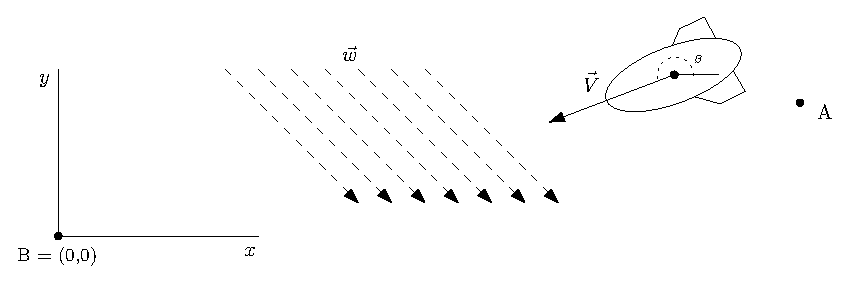
\includegraphics[width=15cm]{figures/airship.eps}
  \caption{Nastínění uvažované situace.}
  \label{Rplot1-2}
\end{figure}

Pro okamžitou rychlost vzducholodi platí:
\begin{equation} 
\label{rce1}
\begin{split}
\dd{x}{t} & = V \cos \beta(t) + u(x,y), \\
\dd{y}{t} & = V \sin \beta(t) + v(x,y),
\end{split}
\end{equation}

kde $
\vec{x}(t)=\transpose{
  \begin{bmatrix}
    x(t) &
    y(t)
  \end{bmatrix}
}
$ je hledaná trajektorie, $\beta \in \langle 0, 2 \pi)$ je směr letu a $
\vec{w}
=
\transpose{
  \begin{bmatrix}
    u &
    v
  \end{bmatrix}
}
$ je dané pole větru. Dále známe:
\begin{subequations}
  \label{eq:1}
  \begin{align}
    \label{eq:2}
    \vec{x}(t_{A})& = A, \\
    \label{eq:3}
    \vec{x}(t_{B})& = B = \transpose{
  \begin{bmatrix}
    0 &
    0
  \end{bmatrix}
},
  \end{align}
\end{subequations}
kde $t_{A}$ je čas startu vzducholodi a $t_{B}$ je čas příletu\footnote{Při příletu vzducholoď nebude mít nulovou rychlost.}. 

\section{Variační počet}
\label{sec:Variační počet}

Náš zájem se proto soustřeďuje na minimalizaci funkcionálu:
\begin{equation}
  \label{eq:8}
  I(\beta, t_{B}) =_{\bydefinition} \int_{t_{A}}^{t_{B}}\, \diff t = t_{B} - t_{A},
\end{equation}
při splnění soustavy rovnic $\eqref{rce1}$, které kompaktněji přepišme jako:
\begin{equation}
  \label{eq:7}
  \dd{\vec{x}}{t} = \vec{f}(\vec{x}, \beta).
\end{equation}
Chceme tedy minimalizovat cestovní čas a přípustné trajektorie musí splňovat $\eqref{eq:7}$. Při hledání extremály využijme koncept vázaných extrémů a Lagrangeových multiplikátorů $\vec{\lambda}$. Proto studujme funkcionál:
\begin{equation}
  \label{eq:9}
  J(\beta, t_{B}) =_{\bydefinition}
  \int_{t = t_{A}}^{t_{B}}
  \left(
    1
    -
    \vectordot{\greekvec{\lambda}}{\left(\dd{\vec{x}}{t} - \vec{f}(\vec{x}, \beta) \right)}
  \right)
  \, \diff t,
\end{equation}
kde funkce $\vec{\lambda}$ bude upřesněna později. Nyní hledejme G\^{a}teauxovu derivaci $J(\beta, t_{B})$:
\begin{equation}
\begin{split}
  \label{eq:13}
  \Diff J(\beta, t_{B}) [(\alpha, \tau)]
  & =
  _{\bydefinition}
  \left.
    \dd{}{\varepsilon}
    J(\beta_{\navext} + \varepsilon \alpha, t_{\navend, \navext} + \varepsilon \tau)
  \right|_{\varepsilon = 0}  \\
  & =
  _{\bydefinition}
  \left.
    \left[
      \dd{}{\varepsilon}
      \int_{t = t_{A}}^{t_{\navend, \navext} + \varepsilon \tau}
      \left(
        1
        -
        \vectordot{\greekvec{\lambda}}{\left(\dd{\vec{x}_{\varepsilon}}{t} - \vec{f}(\vec{x}_{\varepsilon}, \beta) \right)}
      \right)
      \, \diff t
    \right]
  \right|_{\varepsilon = 0}
  ,
\end{split}
\end{equation}
při variaci:
\begin{subequations}
  \label{eq:10}
  \begin{align}
    \label{eq:11}
    \beta &= \beta_{\navext} + \varepsilon \alpha, \\
    \label{eq:12}
    t_{\navend} &= t_{\navend, \navext} + \varepsilon \tau,
  \end{align}
\end{subequations}
kde $\vec{x}_{\epsilon}$ je korespondující trajektorie k $\beta$ a $t_{B}$. Přičemž stále platí:
\begin{subequations}
  \label{eq:010}
  \begin{align}
    \label{eq:020}
    \vec{x}_{\epsilon}(t_{A})& = \vec{x}_{\navext}(t_{A})=A, \\
    \label{eq:030}
    \vec{x}_{\epsilon}(t_{\navend, \navext} + \varepsilon \tau) & =\vec{x}_{\navext}(t_{\navend, \navext})= B = \vec{0}.
  \end{align}
\end{subequations}
Nejdříve upravme $\eqref{eq:13}$ pomocí integrace per partes na člen $\vectordot{\greekvec{\lambda}}{\dd{\vec{x}_{\varepsilon}}{t}}$, některé členy budou dle předchozího nulové a dostáváme:
\begin{multline}
  \label{eq:18}
  \Diff J(\beta, t_{B}) [(\alpha, \tau)]
  =
  \left.
    \left[
      \dd{}{\varepsilon}
      \int_{t = t_{\navstart}}^{t_{\navend, \navext}}
      \left(
        1
        +
        \vectordot{\dd{\greekvec{\lambda}}{t}}{\vec{x}_{\varepsilon}}
        +
        \vectordot{\greekvec{\lambda}}{\vec{f}(\vec{x}_{\varepsilon}, \beta)}
      \right)
      \, \diff t
    \right]
  \right|_{\varepsilon = 0}
  +
  \left.
    \left[
      \dd{}{\varepsilon}
      \int_{t = t_{\navend, \navext}}^{t_{\navend, \navext} + \varepsilon \tau}
      \left(
        1
        +
        \vectordot{\dd{\greekvec{\lambda}}{t}}{\vec{x}_{\varepsilon}}
        +
        \vectordot{\greekvec{\lambda}}{\vec{f}(\vec{x}_{\varepsilon}, \beta)}
      \right)
      \, \diff t
    \right]
  \right|_{\varepsilon = 0}
  \\
  =
    \left.
    \left[
      \dd{}{\varepsilon}
      \int_{t = t_{\navstart}}^{t_{\navend, \navext}}
      \left(
        1
        +
        \vectordot{\dd{\greekvec{\lambda}}{t}}{\vec{x}_{\varepsilon}}
        +
        \vectordot{\greekvec{\lambda}}{\vec{f}(\vec{x}_{\varepsilon}, \beta)}
      \right)
      \, \diff t
    \right]
  \right|_{\varepsilon = 0}
  +
\left.
    \left[
        1
        +
        \vectordot{\greekvec{\lambda}}{\vec{f}(\vec{x}_{\navext}, \beta_{\navext})}
    \right]
  \right|_{t = t_{\navend, \navext}}
  \tau.
\end{multline}
Podle \citep{prusa.tuma} použijeme geniální trik:
$\vec{x}_{\varepsilon} \approx \vec{x}_{\navext} + \epsilon \vec{y} + \cdots$, kde zanedbáme členy vyššího řádu a kde $\vec{y}$ je funkce času. Tím dále můžeme upravit první člen v poslední rovnosti $\eqref{eq:18}$:
\begin{align}
    \left.
    \left[
      \dd{}{\varepsilon}
      \int_{t = t_{\navstart}}^{t_{\navend, \navext}}
      \left(
        1
        +
        \vectordot{\dd{\greekvec{\lambda}}{t}}{\vec{x}_{\varepsilon}}
        +
        \vectordot{\greekvec{\lambda}}{\vec{f}(\vec{x}_{\varepsilon}, \beta)}
      \right)
      \, \diff t
    \right]
  \right|_{\varepsilon = 0} =  \int_{t = t_{\navstart}}^{t_{\navend, \navext}}
  \left(
    \vectordot{\left[ \dd{\greekvec{\lambda}}{t} + \transpose{\left. \pd{\vec{f}}{\vec{x}} \right|_{\vec{x} = \vec{x}_{\navext}, \beta = \beta_{\navext}}} \greekvec{\lambda} \right]}{\vec{y}}
    +
    \vectordot{\greekvec{\lambda}}
    {
      \left. \pd{\vec{f}}{\beta} \right|_{\vec{x} = \vec{x}_{\navext}, \beta = \beta_{\navext}} \alpha
    }
  \right)
  \, \diff t.
\end{align}
Nyní můžeme přistoupit k vybrání $\vec{\lambda}$ takové, aby bylo splněno:
\begin{align}
  \label{eq:24}
  \dd{\greekvec{\lambda}}{t} = - \transpose{\left. \pd{\vec{f}}{\vec{x}} \right|_{\vec{x} = \vec{x}_{\navext}, \beta = \beta_{\navext}}} \greekvec{\lambda}
  .
\end{align}
Po dosazení dostáváme výsledný vztah pro G\^{a}teuxovu derivaci:
\begin{equation}
  \label{eq:25}
  \Diff J(\beta, t_{B}) [(\alpha, \tau)]
  =
  \int_{t = t_{\navstart}}^{t_{\navend, \navext}}
  \vectordot{\greekvec{\lambda}}
  {
    \left. \pd{\vec{f}}{\beta} \right|_{\vec{x} = \vec{x}_{\navext}, \beta = \beta_{\navext}} \alpha
  }
  \, \diff t
  +
  \left.
    \left[
        1
        +
        \vectordot{\greekvec{\lambda}}{\vec{f}(\vec{x}_{\navext}, \beta_{\navext})}
    \right]
  \right|_{t = t_{\navend, \navext}}
  \tau =0
  ,
\end{equation}
což musí platit pro libovolné $\alpha$ a $\tau$. Tímto dostáváme:
\begin{subequations}
  \label{eq:rce2}
  \begin{align}
    \label{eq:31}
    \vectordot{\greekvec{\lambda}}
    {
    \pd{\vec{f}}{\beta}(\vec{x}_{\navext}, \beta_{\navext}) 
    }
    &=
      0, \\
    \label{eq:32}
    \left.
    \left[
    1
    +
    \vectordot{\greekvec{\lambda}}{\vec{f}(\vec{x}_{\navext}, \beta_{\navext})}
    \right]
    \right|_{t = t_{\navend, \navext}}
    &=
      0.
  \end{align}
\end{subequations} 
Pokusme se vypočítat časovou derivaci funkce $1 +  \vectordot{\greekvec{\lambda}}{\vec{f}(\vec{x}_{\navext}, \beta_{\navext})}$, kam dosadíme z rovnic $\eqref{eq:7},\eqref{eq:31}$ a $\eqref{eq:24}$:
\begin{align}
\dd{}{t}
  \left(
    1 +  \vectordot{\greekvec{\lambda}}{\vec{f}(\vec{x}_{\navext}, \beta_{\navext})}
  \right) = 0,
\end{align}
potom funkce $1 +  \vectordot{\greekvec{\lambda}}{\vec{f}(\vec{x}_{\navext}, \beta_{\navext})}$ se musí rovnat konstantě po celý časový interval letu, ale z rovnice $\eqref{eq:32}$ vyplývá, že je rovna nule pro $t \in (t_{A},t_{B})$. Získáváme systém lineárních algebraických rovnic pro $\vec{\lambda}$:
\begin{subequations}
  \label{eq:40}
  \begin{align}
    \label{eq:41}
    1
    +
    \vectordot{\greekvec{\lambda}}{\vec{f}(\vec{x}_{\navext}, \beta_{\navext})}
    &=
      0
      ,
    \\
    \label{eq:42}
    \vectordot{\greekvec{\lambda}}
    {
    \pd{\vec{f}}{\beta}(\vec{x}_{\navext}, \beta_{\navext}) 
    }
    &=
      0.
  \end{align}
\end{subequations}
Řešením této soustavy pro naší pravou stranu $\eqref{rce1}$ můžeme získat explicitní vzorec pro $\vec{\lambda}$:
\begin{equation}
  \label{eq:45}
  \begin{bmatrix}
    \lambda_x \\
    \lambda_y
  \end{bmatrix}
  =
  \frac{1}{V +  u(x_{\navext}, y_{\navext}) \cos \beta_{\navext} +  v(x_{\navext}, y_{\navext}) \sin \beta_{\navext}}
  \begin{bmatrix}
    \cos \beta_{\navext} \\
    \sin \beta_{\navext}
  \end{bmatrix}
  .
\end{equation}
Odkud lze odvodit Zermelova navigační rovnice\footnote{Ernst Zermelo - přednáška v Praze 1931} s použitím rovnice $\eqref{eq:24}$ a užitím skalárního součinu obou stran rovnice s vektorem $
  \transpose{
  \begin{bmatrix}
    -\sin \beta_{\navext} &
     \cos \beta_{\navext}
  \end{bmatrix}
  }
$. Na otázku jak se vyvíjí optimální směr letu vzducholodě $\beta_{\navext}$, nám právě odpovídá Zermelova navigační rovnice:
\begin{equation}
  \label{eq:50}
  \dd{\beta_\navext}{t}
  =
  \pd{v}{x}(x_{\navext}, y_{\navext})
  \sin^2 \beta_\navext
  +
  \left(
    \pd{u}{x}(x_{\navext}, y_{\navext})
    -
    \pd{v}{y}(x_{\navext}, y_{\navext})
  \right)
  \sin \beta_\navext
  \cos \beta_\navext
  -
  \pd{u}{y}(x_{\navext}, y_{\navext})
  \cos^2 \beta_\navext
  .
\end{equation}
Tímto jsme odvodili všechny evoluční rovnice našeho problému.

\section{Řešení}
\label{sec:Řešení}

Máme zadané rychlostní pole větru $\vec{w}$, známe počáteční bod A a koncový bod B letu:
\begin{align}
\vec{w}
& =
\begin{bmatrix}
    u(x,y) \\
    v(x,y)
  \end{bmatrix}
,\\
A
& =
  \begin{bmatrix}
    A_{1} \\
    A_{2} \end{bmatrix}
,\\
B
& =
  \begin{bmatrix}
    0 \\
    0 \end{bmatrix}
.
\end{align}
Optimální trajektorii $\vec{x}_{\navext}$ a nejkratší možný čas letu $t_{B}-t_{A}$ hledáme řešením diferenciálních rovnic:
\begin{subequations}
  \label{eq:51}
  \begin{align}
    \label{eq:52}
    \dd{x_{\navext}}{t} &= V \cos \beta_{\navext} + u(x_{\navext}, y_{\navext}),  \\
    \label{eq:53}
    \dd{y_{\navext}}{t} &= V \sin \beta_{\navext} + v(x_{\navext}, y_{\navext}),  \\
    \label{eq:54}
      \dd{\beta_\navext}{t}
                              &=
  \pd{v}{x}(x_{\navext}, y_{\navext})
  \sin^2 \beta_\navext
  +
  \left(
    \pd{u}{x}(x_{\navext}, y_{\navext})
    -
    \pd{v}{y}(x_{\navext}, y_{\navext})
  \right)
  \sin \beta_\navext
  \cos \beta_\navext
  -
  \pd{u}{y}(x_{\navext}, y_{\navext})
  \cos^2 \beta_\navext
    ,
  \end{align}
\end{subequations}
pro neznámé $\vec{x}_{\navext}=
  \transpose{
  \begin{bmatrix}
    x_{\navext} &
    y_{\navext}
  \end{bmatrix}
  }
$ a $\beta_{\navext}$ při splnění podmínek:
\begin{align}
  \vec{x}_{\navext}(t_{A}) & = A ,\\
  \label{rce3}
  \vec{x}_{\navext}(t_{\navend} ; \beta_{\navext, 0}) & = \vec{0},
\end{align}
kde $\beta_{\navext}(t_{A})=\beta_{\navext, 0}$ je počáteční natočení vzducholodě. Neboli abychom mohli řešit soustavu diferenciálních rovnic $\eqref{eq:51}$, potřebujeme navíc kromě znalosti $\eqref{eq:1}$ ještě přidat další počáteční podmínku $\beta_{\navext, 0}$, pro kterou platí pouze rovnost $\eqref{rce3}$.

Jak si ukážeme v další sekci, pro vhodně zadané rychlostní pole větru lze napsat soustavu rovnic mezi $\vec{x}_{\navext}(t_{A})$ a $ \beta_{\navext, 0}$.

\section{Jednoduché veterné pole}
\label{sec:JVP}
Najjednoduchší prípad veterného poľa, by sme mohli uvažovať bezvetrie. V takom prípade bude pole charakterizované funkciami: $u(x,y)=0$, $v(x,y)=0$. Potom:
\begin{align}
\dd{\beta_\navext}{t} = 0,
\end{align}
z toho:
\begin{align}
\beta_\navext =\beta_{\navext,0},
\end{align}
čo znamená, že vzducholoď bude natočená priamo na cieľ.

Uvažujme teraz prípad lineárnej závislosti veterného poľa na polohe. V tomto prípade bude pole charakterizované funkciami:
\begin{align}
u &= -\frac{V}{h}y ,\\
v &= 0.
\end{align}

\begin{figure}
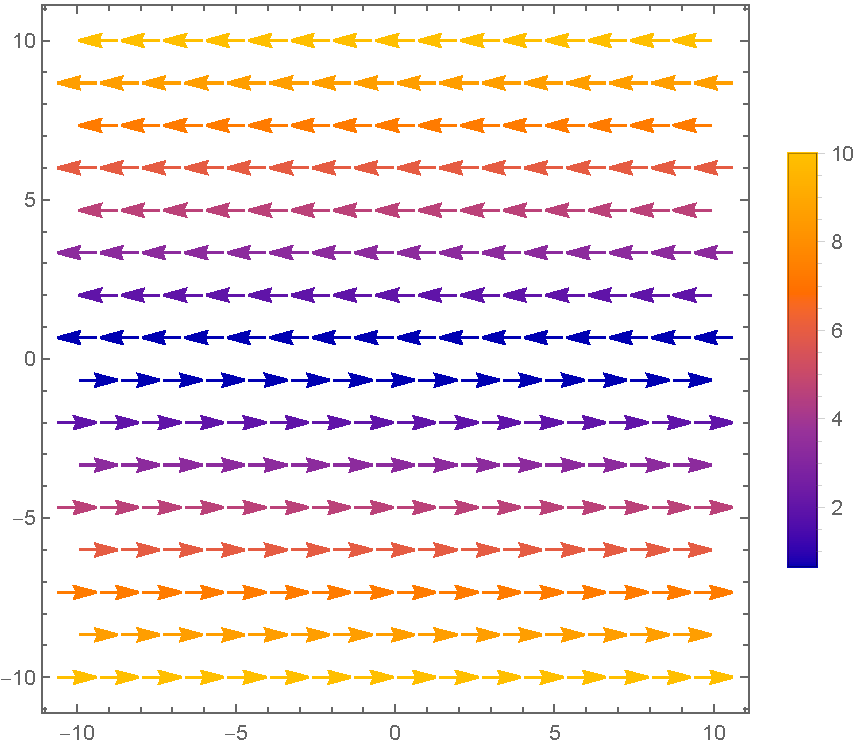
\includegraphics[scale=0.7]{figures/Vekt.pole.pdf}
\caption{Rychlostní pole větru.}
\label{pole}
\end{figure}

Pre tento špeciálny prípad veterného poľa sa systém diferenciálnych rovíc zjednoduší na:
\begin{subequations}
 \label{eq:55}
 \begin{align}
  \label{eq:56}
  \dd{x_{\navext}}{t} &= V \cos \beta_{\navext} - \frac{V}{h}y,  \\
  \label{57}
  \dd{y_{\navext}}{t} &= V \sin \beta_{\navext},  \\
  \label{58}
  \dd{\beta_\navext}{t}
                              &=
  \frac{V}{h}  \cos^2 \beta_\navext.                         
 \end{align}

\end{subequations}
Poslednú rovnicu vieme vyriešiť separáciou premenných:
\begin{align}
 \label{eq:59}
\tan \beta_\navext - \tan \beta_{\navext, B} &= \frac{V}{h}(t-t_{B}),
\end{align}
kde sme použili značenie  $ \left. \beta_{\navext, B}=_{\bydefinition} \beta_{\navext} \right|_{t=t_{\navend, \navext}}   $.  Nakoľko je funkcia $\beta_\navext$ rastúca funkcia času, môžeme zmeniť premenné a prepísať rovnicu \ref{57} ako $\dd{y_{\navext}}{\beta_\navext}\dd{\beta_\navext}{t} = V \sin \beta_\navext$, z čoho dostávame:
\begin{align}
\dd{y_\navext}{\beta_\navext}=h\frac{\sin \beta_\navext}{\cos ^2 \beta_\navext}.
\end{align}
Z toho jednoducho:
\begin{align}
 \label{eq:60}
y_\navext(\beta_\navext)=h\left(\frac{1}{\cos \beta_\navext}-\frac{1}{\cos \beta_{\navext,B}}\right).
\end{align}
Potrebujeme $y_\navext(\beta_{\navext,B})=0$. Nakoniec môžeme uskutočniť rovnakú zmenu premenných v \ref{eq:56}, čo dáva:
\begin{align}
\dd{x_\navext}{\beta_\navext}=h\left(\frac{1}{\cos \beta_\navext}-\frac{1}{\cos^3 \beta_\navext}+\frac{1}{\cos^2 \beta_\navext \cos \beta_{\navext,B}}\right).
\end{align} 
Riešenie v tvare:
\begin{align}
 \label{eq:61}
x_\navext(\beta_\navext)=\frac{1}{2}h(-\arctanh \sin \beta_{\navext,B} + \arctanh \sin \beta_\navext - \sec \beta_{\navext,B} \tan \beta_{\navext,B} + 2\sec \beta_{\navext,B} \tan \beta_\navext - \sec \beta_\navext \tan \beta_\navext),
\end{align}
potrebujeme aby platilo $x_\navext(\beta_{\navext,end})=0$. Teraz môžeme použiť rovnice \ref{eq:61} a \ref{eq:60}. Počiatočné podmienky musia vyhovovať \ref{eq:2}, teda dostávame systém rovníc:
\begin{align}
 \label{eq:62}
\vec{x}(t_{A})
=
\begin{bmatrix}
    \frac{1}{2}h(-\arctanh \sin 	       \beta_{\navext,B} + \arctanh \sin \beta_\navext - \frac{1}{\cos \beta_{\navext,B}} \tan \beta_{\navext,B} + \frac{2}{\cos \beta_{\navext,B}} \tan \beta_\navext - \frac{1}{\cos \beta_\navext} \tan \beta_\navext) \\
    h\left(\frac{1}{\cos \beta_\navext}-\frac{1}{\cos \beta_{\navext,B}}\right)
  \end{bmatrix}.
\end{align}
Nakoľko poznáme $\vec{x}(t_{A})$, dostávame teda z \ref{eq:62} sústavu dvoch nelineárnych algebraických rovníc pre dve neznáme $\beta_{\navext,end}$ a $\beta_\navext$. Akonáhle nájdeme tieto dve hodnoty, môžeme z rovnice \ref{eq:59} vyjadriť konečný čas.

Konečne môžeme konštatovať, že pre výpočet úlohy navigácie lode, potrebujeme pre dané $V$, $h$ a 
$\vec{x}(t_{A})= \transpose {\begin{bmatrix}
    x(t_{A}) &
    y(t_{A})
  \end{bmatrix}
},
$
vyriešiť systém nelineárnych algebraických rovníc:
\begin{align}
 \label{eq:63}
\begin{bmatrix}
x(t_{A})\\
y(t_{A})
\end{bmatrix}
=
\begin{bmatrix}
    \frac{1}{2}h(-\arctanh \sin 	       \beta_{\navext,B} + \arctanh \sin \beta_\navext - \frac{1}{\cos \beta_{\navext,B}} \tan \beta_{\navext,B} + \frac{2}{\cos \beta_{\navext,B}} \tan \beta_\navext - \frac{1}{\cos \beta_\navext} \tan \beta_\navext) \\
    h\left(\frac{1}{\cos \beta_\navext}-\frac{1}{\cos \beta_{\navext,B}}\right)
  \end{bmatrix}
\end{align}
a dostaneme hodnoty $\beta_\navext$ a $\beta_{\navext,B}$. Z rovnice 
\begin{align}
\tan \beta_{\navext,A} - \tan \beta_{\navext, B} &= \frac{V}{h}(t_{A}-t_{B}),
\end{align}
nájdeme konečný čas $t_{B}$. Optimálna trajektória je daná ako riešenie systému diferenciálnych rovníc prvého stupňa:
\begin{subequations}
 \label{eq:64}
 \begin{align}
  \label{eq:65}
  \dd{x_{\navext}}{t} &= V \cos \beta_{\navext} - \frac{V}{h}y_\navext,  \\
  \label{eq:66}
  \dd{y_{\navext}}{t} &= V \sin \beta_{\navext},  \\
  \label{eq:67}
  \dd{\beta_\navext}{t}
                              &=
  \frac{V}{h}  \cos^2 \beta_\navext, 
 \end{align}
\end{subequations}
ktoré sa riešia v časovom intervale $t \in (t_{A}, t_{B})$, s ohľadom na počiatočné podmienky:
\begin{subequations}
 \label{eq:68}
 \begin{align}
  \label{eq:69}
  \left. x_\navext \right|_{t=t_{A}} &= x_{A},  \\
  \label{eq:70}
  \left. y_\navext \right|_{t=t_{A}} &= y_{A},   \\
  \label{eq:71}
  \left. \beta_\navext \right|_{t=t_{A}} &= \beta_{\navext, A}. 
 \end{align}
\end{subequations}
Problém \ref{eq:63} až \ref{eq:68} sa dá vyriešiť numerickými metódami.

\section{Numerické řešení}
\label{sec:NumJVP}
Jak jsme už naznačili, naše jednoduché větrné pole se dá vyřešit numericky\footnote{Veškeré výpočty jsou provedeny v programu Wolfram Mathematica, verze 12.2.}. Rozhodli jsme se pracovat s následujícími hodnotami\footnote{Naše hodnoty mají následující jednotky: $V$ a $"h1-h3"$ - \si{km.h^{-1}}, $x1$ a $x2$ - \si{km}.}:
\begin{lstlisting}[language=Mathematica, caption=Hodnoty]
V = 10;
h1 = 1;
h2 = 10;
h3 = 0.1;
x1 = "in. condition X";
x2 = "in. condition Y"
\end{lstlisting}

Pro rychlost vzducholodě $V$ jsme si brali jen jednu hodnotu. Při našich výpočtech se ukázalo, že různé hodnoty $V$ nemají vliv na trajektorii, takže ani na startovní úhel $\beta_{ext,A}$. Ovlivněna je jen doba letu.

Nazveme x-ovou část vektoru \eqref{eq:63} $X1$ a y-ovou část stejného vektoru $X2$. Za $x(t_{A})$ dáme $x1$ a za $y(t_{A})$ dáme $x2$. Získáme dvě rovnice: $X1=x1$ a $X2=x2$. V těchto rovnicích se nachází hodnota $h$, za kterou postupně dosazujeme hodnoty $"h1-h3"$. Pojďme vyřešit tuto soustavu nelineárních algebraických rovnic.

Pro numerické řešení použijeme metodu $FindRoot$. 
 
\begin{lstlisting}[language=Mathematica, caption=Metoda řešení,mathescape]
res = FindRoot[{X1 == x1, X2 == x2}, {{B1, "0-2$\pi$"}, {B2, "0-2$\pi$"}}]
\end{lstlisting}

Metoda \texttt{FindRoot} byla jediná, která v našich výpočtech fungovala. Bohužel je v tomto případě ne až tak praktická, kvůli dlouhému hledání nejvhodnějších parametrů $B1$ a $B2$.

Řešení \eqref{eq:63} můžeme pak použijeme k výpočtu času, za který se dostane vzducholoď z bodu A do bodu B.

\begin{lstlisting}[language=Mathematica, caption=Výpočet času,mathescape]
$\beta_{ext,A}$ = B1 /.res;
$\beta_{ext,B}$ = B2 /.res;
time = -(h/V)(Tan[$\beta_{ext,A}$] - Tan[$\beta_{ext,B}$])
\end{lstlisting}

Nakonec si vykreslíme trajektorie.
\begin{lstlisting}[language=Mathematica, caption=Vykreslení trajektorie,mathescape]
rce = {x'[t] == V*Cos[$\beta$[t]] - (V/"h1-h3")y[t];
y'[t] == V*Sin[$\beta$[t]];
$\beta$'[t] == (V/"h1-h3")(Cos[$\beta$[t]])^2};

sol = NDSolve[Join[rce, {x[0] == x1, y[0] == x2, $\beta$[0] == $\beta_{ext,A}$], {x, y, $\beta$},{t, 0, 3600}];

ParametricPlot[Table[{x[t], y[t]} /. sol], {t, 0, time}, AxesLabel -> {x, y}, PlotRange -> All]
\end{lstlisting}


\subsection{Osa X}
\label{sec: OsaX}

\begin{wrapfigure}{r}{.55\textwidth}
    \begin{minipage}{\linewidth}
    \centering
    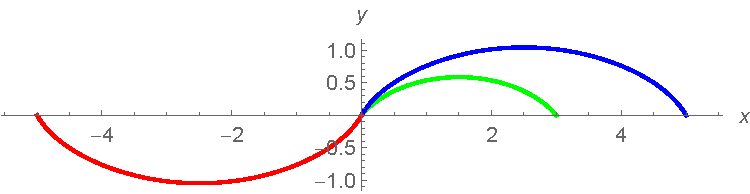
\includegraphics[width=10cm]{figures/OsaX2.pdf}
    \caption{Trajektorie, start osa $x$, $h$ = 1}
    \label{Xtraj1}
    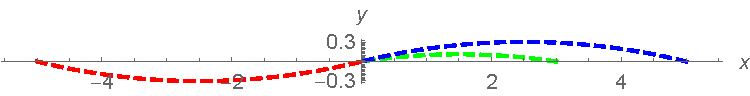
\includegraphics[width=10cm]{figures/OsaX3.pdf}
    \caption{Trajektorie, start osa $x$, $h$ = 10}
    \label{Xtraj10}
    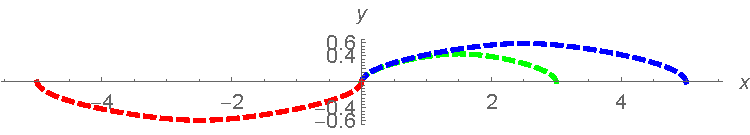
\includegraphics[width=10cm]{figures/OsaX4.pdf}
    \caption{Trajektorie, start osa $x$, $h$ = 0.1}
    \label{Xtraj0.1}
    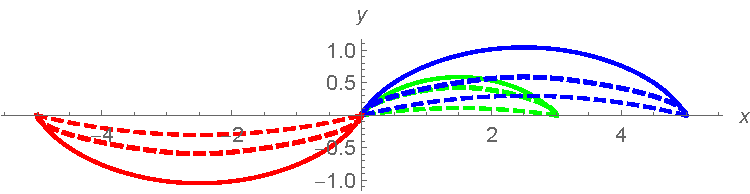
\includegraphics[width=10cm]{figures/OsaX1.pdf}
    \caption{Trajektorie, start osa $x$}
    \label{Xtraj}
\end{minipage}
\end{wrapfigure}

Začneme s případem - start z osy $x$.

Startujeme tak, že vplujeme do větrného pole z bezvětří a pomalu/rychle se necháme unášet k našemu cíli. Tento případ je nejintuitivnější. Zhruba si dokážeme představit trajektorii, podél které se vzducholoď pohybuje.

Pro lepší představu se můžeme podívat na obrázky \eqref{Xtraj1}, \eqref{Xtraj10} a \eqref{Xtraj0.1}, kde vykreslujeme trajektorie pro různé hodnoty $h$. Pro porovnání těchto trajektorií se můžeme kouknout na obrázek \eqref{Xtraj}. V tabulce \eqref{TabX1} máme délku doby letu v hodinách a v tabulce \eqref{TabX2} máme startovní úhel v radiánech.

\subsection{Osa Y}
\label{sec: OsaY}

Koukneme se na start z osy $y$.

Tento případ začíná být už zajímavější. Pro velká $h$ a malá $y$ je trajektorie podobná trajektorii, která začíná z osy $x$. Na obrázku \eqref{Ytraj} lze pozorovat, že čím je $y$ dále od počátku, tak se trajektorie protahuje. Toto samé platí, když hodnotu $h$ snižujeme, což lze pozorovat na obrázku \eqref{Ytraj0.1}. V tabulkách \eqref{TabY1} a \eqref{TabY2} máme časy a startovní úhly pro různé pozice. Když porovnáme časy, které jsem získali při studování startů z osy $x$ a osy $y$, můžeme si všimnout, že jsme zpravidla rychleji v cíli, když startujeme z osy $x$. 
\subsection{Kvadranty}
\label{sec: Kvad}
Zamíříme k obecnějšímu případu - start z kvadrantů.

Vybrali jsme jen tři různé počáteční podmínky ze dvou kvadrantů (1. a 2.). Proč jen ze dvou kvadrantů? Jak jsme mohli vypozorovat ze startů z os $x$ a $y$, tak trajektorie jsou středově souměrná podle počátku (pokud je i jejich počáteční startovní bod středově souměrný podle počátku)\footnote{Tato vlastnost plyne ze symetrie větrného pole - je také středově souměrné podle počátku.}, takže není nutné studovat chování v 3. a 4. kvadrantu.

Na obrázku \eqref{Ktraj1} můžeme pozorovat, jak se mění tvary trajektorií v závislosti na počátečních podmínkách. Na obrázku \eqref{Ktraj10} lze vidět, že když zvětšíme $h$, tak trajektorie budou mít tendenci mířit přímo do cíle. V tabulkách \eqref{TabK1} a \eqref{TabK2} uvádíme zase dobu letu a startovní úhel.


\begin{figure}[h]
  \centering
  \subfloat[Doba letu v hodinách]{
  \label{TabX1}
  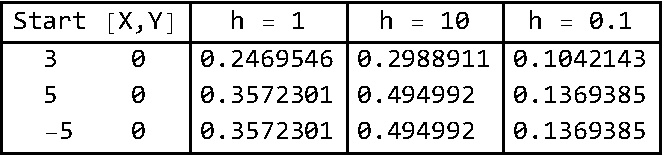
\includegraphics[scale=0.7]{figures/OsaX - tab. čas.pdf}
  }
  \qquad
  \subfloat[Startovní úhel $\beta_{\navext}(t_{A})$  v radiánech]{
  \label{TabX2}
  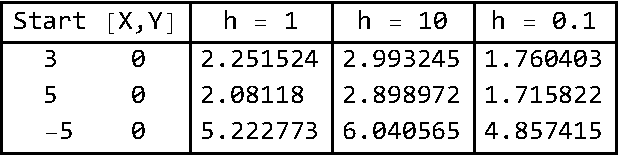
\includegraphics[scale=0.7]{figures/OsaX - tab. beta.pdf}
  }
\caption{Osa $x$}
\end{figure}

\begin{figure}[ht]
  \centering
  \subfloat[$h$ = 1 (nečárkované), $h$ = 10 (čárkované)]{
  \label{Ytraj}
  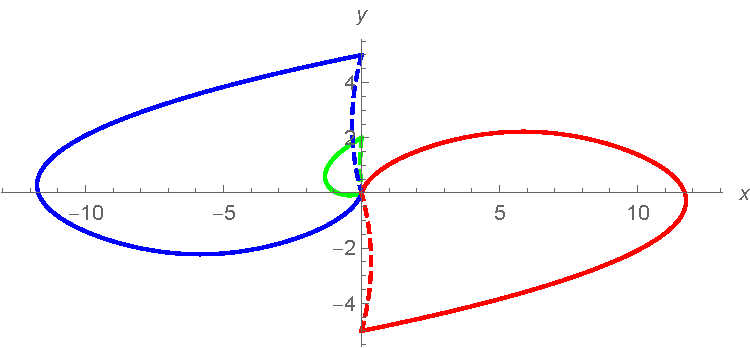
\includegraphics[scale=0.65]{figures/OsaY1.pdf}
  }
  \qquad
  \subfloat[$h$ = 0.1]{
  \label{Ytraj0.1}
  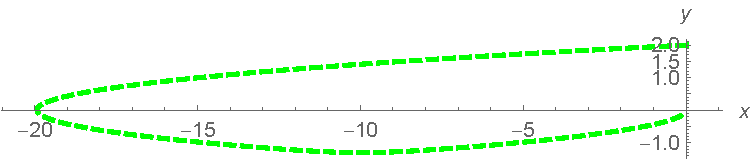
\includegraphics[scale=0.65]{figures/OsaY4.pdf}
  }
  \qquad
  \subfloat[Doba letu v hodinách]{
  \label{TabY1}
  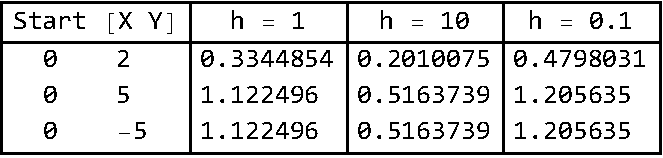
\includegraphics[scale=0.6]{figures/OsaY - tab. čas.pdf}
  }
  \qquad
  \subfloat[Startovní úhel $\beta_{\navext}(t_{A})$  v radiánech]{
  \label{TabY2}
  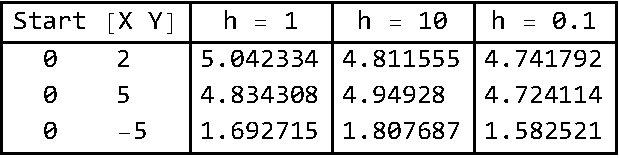
\includegraphics[scale=0.6]{figures/OsaY - tab. beta.pdf}
  }
\caption{Osa $y$}
\end{figure}

\begin{figure}[ht]
  \centering
  \subfloat[$h$ = 1]{
  \label{Ktraj1}
  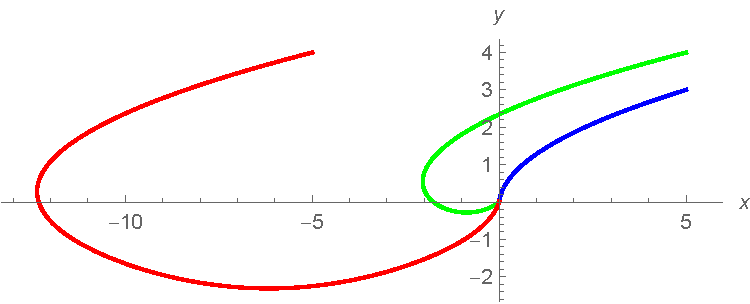
\includegraphics[scale=0.65]{figures/Kvad2.pdf}
  }
  \qquad
  \subfloat[$h$ = 10]{
  \label{Ktraj10}
  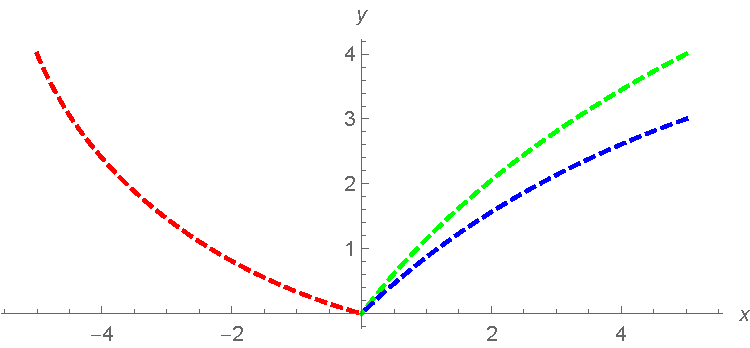
\includegraphics[scale=0.65]{figures/Kvad3.pdf}
  }
  \qquad
  \subfloat[Trajektorie, startů v kvadrantech]{
  \label{Ktraj}
  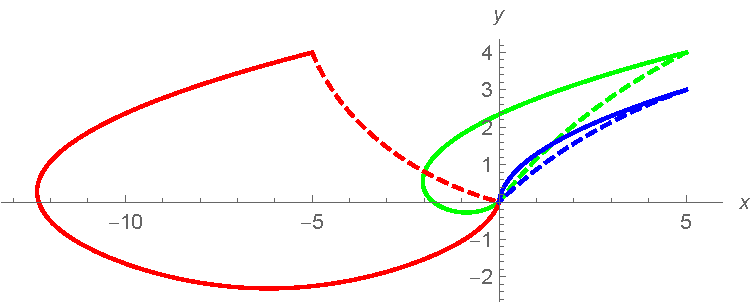
\includegraphics[scale=0.9]{figures/Kvad1.pdf}
  }
  \qquad
  \subfloat[Doba letu v hodinách]{
  \label{TabK1}
  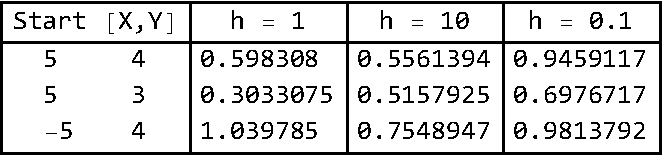
\includegraphics[scale=0.6]{figures/Kvad - tab. čas.pdf}
  }
  \qquad
  \subfloat[Startovní úhel $\beta_{\navext}(t_{A})$  v radiánech]{
  \label{TabK2}
  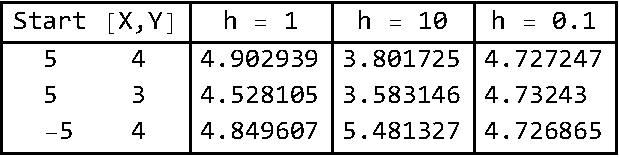
\includegraphics[scale=0.6]{figures/Kvad - tab. beta.pdf}
  }
\caption{Kvadranty}
\end{figure}


%\begin{figure}
%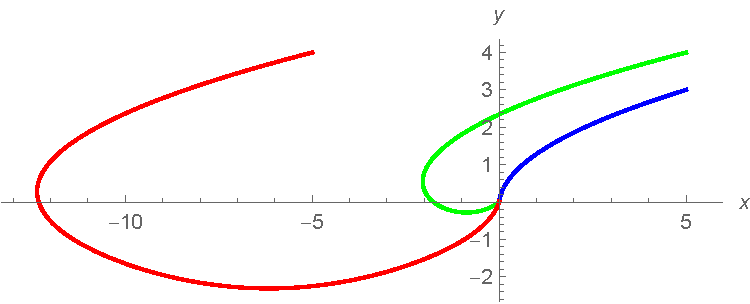
\includegraphics[scale=0.7]{figures/Kvad2.pdf}
%\caption{Trajektorie, start v kvadrantu, $h$ = 1}
%\label{Ktraj1}
%\end{figure}

%\begin{figure}
%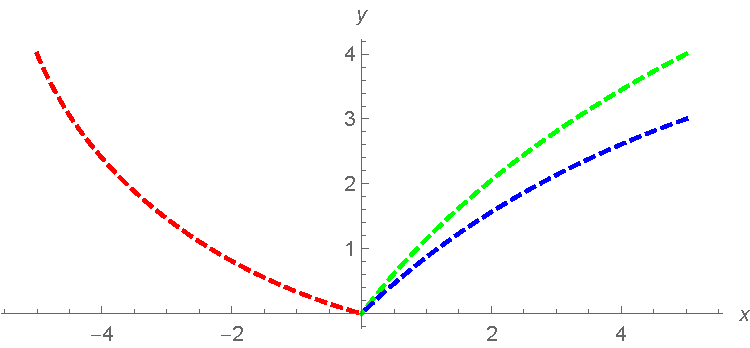
\includegraphics[scale=0.7]{figures/Kvad3.pdf}
%\caption{Trajektorie, start v kvadrantu, $h$ = 10}
%\label{Ktraj10}
%\end{figure}

%\begin{figure}
%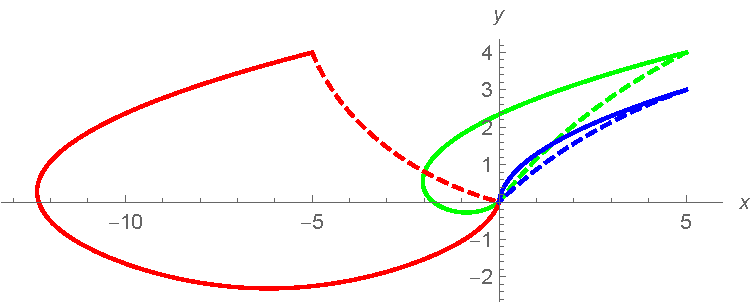
\includegraphics[scale=0.7]{figures/Kvad1.pdf}
%\caption{Trajektorie, start v kvadrantu}
%\label{Ktraj}
%\end{figure}

%\begin{figure}
%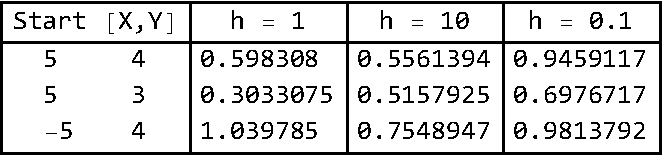
\includegraphics[scale=0.7]{figures/Kvad - tab. čas.pdf}
%\caption{Tabulka - doba letu (hodiny)}
%\label{TabK1}
%\end{figure}
%
%\begin{figure}
%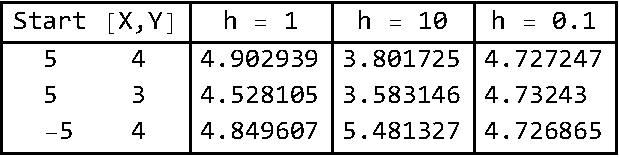
\includegraphics[scale=0.7]{figures/Kvad - tab. beta.pdf}
%\caption{Tabulka - startovní úhel (radiány)}
%\label{TabK2}
%\end{figure}




















%\begin{lstlisting}[language=Mathematica, caption=Konstanty]
%g = 9.81;
%l = 1;
%poc = 1;
%time = {t, 0, 10};
%\end{lstlisting}




\bibliographystyle{custom}
\bibliography{ref}

\addtocontents{toc}{\protect\end{multicols}} % workaround for table of contents in two columns in amsart documentclass
\end{document}

%%% Local Variables: 
%%% mode: latex
%%% TeX-master: t
%%% End: 
